\hypertarget{bug-simulations}{%
\section{Bug simulations}\label{bug-simulations}}

Even though the bug algorithms are intended to illustrate particular
ideas, they are valid algorithms for path planning. In addition,
roboticists get some odd sense of pleasure out of watching planners
succeed. We will restrict our work here to discrete (bitmap) domains
only because it makes the headache of determining collision go away. A
collision requires the robot to move. How is this done?

There are two ways initially you can approach controlling the robot:
through position or velocity. A position control sets the location
directly. The other method, velocity, control adjusts the velocities and
the position is updated indirectly. Position control is easy to start
with when you directly work with the simulation window or canvas. It is
not really how a robot is controlled since it models stop and go motion.
Velocity control follows how most mobile robots are actually controlled.
The movement must be consistent with vehicle kinematics which can vary
depending on robot design. For example a differential drive robot can
set forward velocity and rotational (turn) velocity. Using the kinematic
equations (presented later), position and orientation can be computed.

Earlier we discussed how to determine obstacle impact or collision for a
circular robot. For a general robot shape, impact is more difficult to
compute. Collision can be defined as when the distance between the robot
and obstacle becomes zero. In the continuous world, the distance is

\[D(t) = \min \sqrt{(x_R(t)-x_O)^2 + (y_R(t)-y_O)^2}\]

where \((x_R,y_R)\) lies on the robot boundary and \((x_O,y_O)\) lies on
the object boundary. Setting \(D=0\) and solving for \(t\) then provides
the time and location of the collision. However, the robot and the
obstacle will have some shape defined by a bitmap. Collision between the
robot and the obstacle boils down to determining if a pixel or pixels
will overlap after a robot position update. You might notice that this
is not quite correct. It is possible for the time step to be large
enough that the robot appears to jump over obstacles. In that case, we
need to select a smaller time update so that motion begins to appear
continuous and teleporting robots are avoided.

Assume that you have \(n\) objects in the landscape which have a general
discrete (bitmap) shape. This means each obstacle is a union of squares.
After the motion step, one needs to check if any pixel occupied by the
robot is also occupied by an obstacle. After the move, all of the pixels
associated with the robot location are checked. If any pixel is painted
black, then the robot has driven into an obstacle. This should generate
an event associated with a crash and signal both the graphics window as
well as the control program.

This same approach may be used to simulate a bump or touch sensor. The
boundary pixels of the robot can be used as the sensors. If those pixels
are adjacent to an object, then a touch is registered. This can be done
via a direct adjacency test - looking at neighbor pixels. Or this can be
done by a ghost pixel method. Inflate the objects by one row of pixels.
If the robot overlaps a ghost pixel then the corresponding robot
pixel/sensor would register a touch. Inflation is essentially one step
of a flood fill. Flood fill is normally implemented as a type of DFS
algorithm, but does not need this machinery here. A common error here is
to write the adjacent pixel into the current array, but if you are
sweeping through the image row by row, you might use this new pixel as
an obstacle pixel. Then this new sweep will mark the neighbor. This can
continue and cause lines to grow down with the sweep.

An array used for the image data which stores multiple values can be
very handy. Pixels are marked according to type. For example, zero for
open pixel, one for a robot occupied pixel, two for an obstacle, three
for the inflated set. Later on having data stored per pixel (or cell) is
essential for our motion planners.

\hypertarget{getting-a-map}{%
\subsection{Getting a Map}\label{getting-a-map}}

There are a variety of approaches for getting map data created. Various
range sensors and cameras have been used to create viable maps. Pixel
based occupancy grids are relatively easy to create. For mazes, we might
only be interested in the topology of occupied or free space. A
skeletonization of free space returns a graph that can be used for graph
based search algorithms.

\hypertarget{implementation}{%
\subsection{Implementation}\label{implementation}}

The algorithms presented above have two basic modes. One is motion to
goal. This behavior assumes that the robot knows the target location or
at least knows the direction to head. This is done in practice using a
type of localization system. In a simulated environment, it is of course
very easy since you always have absolute knowledge of the robot and
goal's location. The more challenging problem is boundary following.
Unless you have very accurate maps to start with or apriori knowledge of
the objects in the environment, the boundaries of the obstacles are
unknown. This means they must be discovered during the planning process.
How does the robot move around the boundary? What information is
required? What information is provided by the sensors and so what
information needs to be computed? How is the path determined?

We will assume that object boundaries are smooth curves and would be
locally a function, \(y-f(x)\). If this is the case, we can compute the
tangent and normal directions as shown in \texttt{offsetcurve\_a}. An
offset curve is a curve that follows the boundary at some fixed distance
from the boundary. It looks like a level set curve. We can compute the
tangents and normals for offsets as well, \texttt{offsetcurve\_b}.

\begin{quote}
We assume that the boundary is a smooth function.

The normal and tangent directions to the offset curve.
\end{quote}

An offset curve can be found analytically using only the Tangent
direction vector \(v(t)\) {[}where \(v\) is a basis vector in
\((n(c(t)))^\perp\){]}. Assume that the curve is given in parametric
form \(\{c_1(t), c_2(t)\}\). Solving the differential equations
\(\dot{c}(t) = v\), \(\{c_1(0), c_2(0)\} = c_0\) provides the offset
curve.

\textbf{Example:} If the tangent to an offset curve is \(v = <-y, 2x>\),
find the offset curve \(\dot{c}(t) = v\) when \(c_0 = (1,2)\).

\[\dot{c}(t)=dc/dt = <dx/dt , dy/dt> = <-y,2x>\]

so (1) \(dx/dt = -y\) and (2) \(dy/dt = 2x\). Differentiate the first
equation to get \(d^2x/dt^2 = -dy/dt\) and then plug into the second
equation: \(d^2x/dt^2 = -2x\). We can solve this equation to obtain

\[x(t) = A\cos\sqrt{2}t + B\sin\sqrt{2}t.\]

The condition \(x(0) = 1\) means \(x(0) = A = 1\). From the first
equation we obtain

\[y(t) = \sqrt{2}\sin\sqrt{2}t - B\sqrt{2}\cos\sqrt{2}t\]

Using the second condition, \(y(0)=2\), we see that \(B = -\sqrt{2}\).

We have already discussed computing an obstacle boundary normal and
tangent, \texttt{turtleboundary}, using a ring of touch sensors. In a
real application, you may stop once the tangent has been determined. The
robot can be steered in that direction. The act of driving the robot
continuously in the direction of \(v\) is the same as solving the
differential equations (other than the different errors that arise).

\hypertarget{simple-boundary-following-using-a-range-sensor}{%
\subsubsection{Simple boundary following using a range
sensor}\label{simple-boundary-following-using-a-range-sensor}}

If a range sensor is available, it is a better choice for determining
the boundary normal (avoids contact with the obstacle). Assume that you
are looking to follow the boundary of obstacle 2 in \texttt{rangeinfo}.
Let \(D(x)\) be the distance from \(x\) to the followed obstacle:

\[D(x) = \min_{c\in{\cal W}{\cal O}_i} d(x,c)\]

Look for global minimum to find the point on the followed obstacle. The
gradient of distance is given by

\[\begin{aligned}
\nabla D(x) = \begin{bmatrix} \displaystyle \frac{\partial D(x)}{\partial x_1}\\[5mm]
\displaystyle\frac{\partial D(x)}{\partial x_2}\end{bmatrix}
\end{aligned}\]

The closest point by definition is the point that is a minimum of the
distance function between the ranging device, \(x\), and the obstacle
boundary, \(y\). This means that the tangent must be orthogonal to the
line segment connecting \(x\) and \(y\). Once the direction to \(y\) is
determined then the travel direction can be computed. Assume the
direction to \(y\) is given by \(\nabla D(x) = <a_1,a_2>\). The travel
direction is \(\pm <a_2, -a_1>\) which is orthogonal to \(\nabla D\).

\begin{quote}
Obtaining information from range data.
\end{quote}

A ranging device in practice returns discrete data. You can detect the
approximate nearest point on the obstacle boundary, say at index k in
the range array data: d{[}{]}. You can convert (k-1, d{[}k-1{]}),(k,
d{[}k{]}),(k+1, d{[}k+1{]}) into (x,y) points in the robots coordinates:
\((x_{k-1}, y_{k-1})\), \((x_{k}, y_{k})\), \((x_{k+1}, y_{k+1})\):

\[(x_k,y_k) = \left(d[k] \cos (\Delta \theta k + \theta_0), d[k] \sin (\Delta \theta k + \theta_0)\right)\]

where \(\theta_0\) is the angle for the start of the sweep. Knowing the
closest point on the boundary to the robot is again sufficient to
compute the tangent direction. We can smooth out the boundary motion
using algorithm~\href{alg:boundarymotion}{Boundary Motion}

\begin{quote}
List all neighbor cells adjacent to occupied cells.\\
Select neighbor according to policy (right or left hand travel):
(m,n).\\
Mark (i,j) as visited.\\
Set current cell: (m,n) \(\to\) (i,j).\\
\textbf{while} Not arrived at leave point \textbf{do}\\
\hspace*{0.333em}\hspace*{0.333em}*\emph{repeat}*\\
\hspace*{0.333em}\hspace*{0.333em}\hspace*{0.333em}\hspace*{0.333em}List
unvisited neighbor cells adjacent to occupied cells.\\
\hspace*{0.333em}\hspace*{0.333em}\hspace*{0.333em}\hspace*{0.333em}Select
neighbor: \{tt (m,n)\}\\
\hspace*{0.333em}\hspace*{0.333em}\hspace*{0.333em}\hspace*{0.333em}Mark
\{tt (i,j)\} as visited.\\
\hspace*{0.333em}\hspace*{0.333em}\hspace*{0.333em}\hspace*{0.333em}Set
current cell: \{tt (m,n)\} \$to\$ \{tt (i,j)\}.\\
\hspace*{0.333em}\hspace*{0.333em}*\emph{end while}*
\end{quote}

\hypertarget{image-coordinates-and-coordinates}{%
\subsubsection{Image coordinates and
coordinates}\label{image-coordinates-and-coordinates}}

Images are simply two dimensional arrays of integers. Much like matrices
in your math courses. There are a couple of differences you need to
know. First, the coordinate system for an image has the y coordinate
increasing as you head down. Second, the origin is the top left pixel.
The graphic below indicates this coordinate system. The way we store two
dimensional arrays is Array{[}row{]}{[}col{]}. Increasing row will
increase in the y direction downwards. So the two dimensional array is
consistent with the image coordinate system. We will call neighbor
pixels the eight pixels surrounding the center pixel. The graphic below
shows the standard mathematical notation for plots and graphs \((x,y)\)
and the array notation for the pixels.

\begin{figure}
\centering
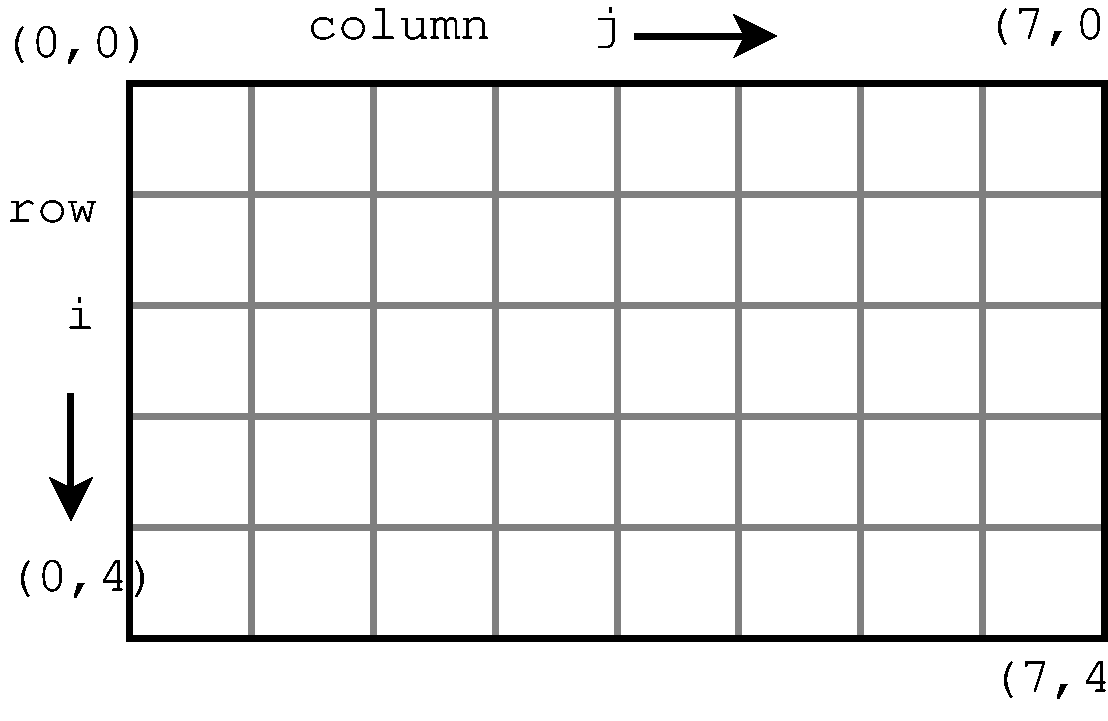
\includegraphics[width=0.5\textwidth,height=\textheight]{NavigationFigures/imagecoords.*}
\caption{}
\end{figure}

\begin{figure}
\centering
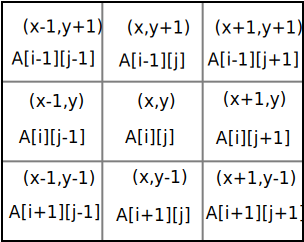
\includegraphics[width=0.5\textwidth,height=\textheight]{NavigationFigures/neighbors.*}
\caption{}
\end{figure}

\hypertarget{c-easy-access-of-neighbor-pixels}{%
\subsection{C++ easy access of neighbor
pixels}\label{c-easy-access-of-neighbor-pixels}}

Assume that you have an image stored in the two dimensional array map.
Many algorithms require you to access all eight neighbor pixels. You can
write these out by hand or you can do a two dimensional loop. The
following code accesses all eight neighbors and the point itself (nine
pixels):

\begin{verbatim}
for(i=-1;i<=1;i++) {
     for(j=-1;j<=1;j++) {
           value = map[row+i][col+j];
      }
}
\end{verbatim}

Most likely your implementation will not care about the center point.
But if you explicitly want to skip it, try adding a
conditional\footnote{\texttt{if((i!=0)\textbar{}\textbar{}(j!=0))}}. Be
very careful about stepping outside map array bounds. Either you need to
check for stepping outside the array or your loops need to stay inside
the array. For example, instead of running \(i=0\) to \(i=n\) you run
from \(i=1\) to \(i=n-1\). The outer layer of pixels are the ``walls"
and you don't touch them. This is why we suggest having a layer or two
of black pixels around the map.

\hypertarget{impacts-in-grid-environments}{%
\subsection{Impacts in grid
environments}\label{impacts-in-grid-environments}}

The last issue that needs to be addressed is object interaction. How
should we handle an impact? In \texttt{Fig:RobotSize}, we saw that for
circular robots, we could just add the radius of the robot to the
obstacle and then treat the robot as a point mass. For path planning of
circular robots we can then inflate the obstacle using a truncated flood
fill algorithm and proceed with path planning using just a point as the
robot. The flood fill algorithm will be discussed later on in this
chapter. We can then assume that all of the obstacle maps have been
preprocessed and just focus on the planning aspect.

Detecting a collision is now very easy. The robot is a point and so
impact is determined if the point is adjacent to an obstacle. Assume
that the robot is at location and the obstacle map is obstMap{[}i,j{]}.
Also assume that empty space is represented by 0 in the array, filled
space is represented by 1, and the boolean variable impact records
impact or not.

\begin{verbatim}
if (obstMap[i+1,j] == 1) or (obstMap[i-1,j] == 1) or \
        (obstMap[i,j+1]== 1)  or (obstMap[i,j-1]== 1) :
    impact = 1
\end{verbatim}

This will work to determine if is adjacent to a filled pixel. The
problem that arises is with the array boundaries. For example if i = 0
then the comparison obstMap{[}i-1,j{]} == 1 falls out of the array
bounds. The literature has two standard approaches for this issue. One
way to proceed is to treat the four sides and four corners of the array
as special cases with code lines of the form if i == 0 then omit the
left neighbor check. One must do this for top and bottom, left and right
boundaries.

The second common approach in the literature is known as ghost points.
The idea is to inflate the array by one pixel on each boundary. Say that
the obstacle map is 800 wide x 600 high. Normally your array runs i =
0..799 and j = 0..599. Declare the storage array to be 802 x 602. Then
place the obstacle map in i = 1..800 x j = 1..600. We define an open
landscape as no solide boundary on the edges of the obstacle map
(meaning no walls around the region). A closed landscape will have
walls. For an open landscape set the arrray entries for , {[}i =
801,j{]} , {[}i, j=0{]} , {[}i,j = 601{]} equal to zero. For a closed
landscape set those values to 1. The boundaries no longer generate out
of array errors and the need for special boundary cases is eliminated.
The code above will work as is.

The simplest approach is to flood fill about the obstacle the full
radius plus one. This means that when the center of the robot overlaps
the obstacle on the configuration space, the physical robot is adjacent
in the physical workspace. It neither requires a list of comparisons or
an inflated array. In this case the code is very simple:

\begin{verbatim}
if (obstMap[i,j] == 1):
    impact = 1
\end{verbatim}

It is now time to put everything together. We first list the server code
example. As above, a few lines have a backslash continuation character
which are for typesetting here and are not needed in the code. For
simplicity the obstacle map will use 0 for occupied and not 0 for open.
These just follows the image where black is 0 and which is 255. The code
first sets up the Turtle canvas. It places the robot at (-300,0) and
selects not to draw the path. Then we take a break and setup the
sockets. The program will block until a socket is established (recall
the discussion on event loops). Finally the progam enters the turtle
loop. It reads a comment on the socket and then issues that command to
the Turtle. The client program discussed above is used to communicate
with the turtle server.

The impact aspect is not really robust. The focus is on planning, not on
physics. We make no attempt to stop the robot and allow it to pass
through walls. It is the responsibility of the planner to stop, backup,
turn and move around.

\textbf{Footnotes}
